\documentclass[]{article}
\usepackage[left=1in,top=1in,right=1in,bottom=1in]{geometry}


%%%% more monte %%%%
% thispagestyle{empty}
% https://stackoverflow.com/questions/2166557/how-to-hide-the-page-number-in-latex-on-first-page-of-a-chapter
\usepackage{color}
% \usepackage[table]{xcolor} % are they using color?

% \definecolor{WSU.crimson}{HTML}{981e32}
% \definecolor{WSU.gray}{HTML}{5e6a71}

% \definecolor{shadecolor}{RGB}{248,248,248}
\definecolor{WSU.crimson}{RGB}{152,30,50} % use http://colors.mshaffer.com to convert from 981e32
\definecolor{WSU.gray}{RGB}{94,106,113}

%%%%%%%%%%%%%%%%%%%%%%%%%%%%

\newcommand*{\authorfont}{\fontfamily{phv}\selectfont}
\usepackage{lmodern}


  \usepackage[T1]{fontenc}
  \usepackage[utf8]{inputenc}




\usepackage{abstract}
\renewcommand{\abstractname}{}    % clear the title
\renewcommand{\absnamepos}{empty} % originally center

\renewenvironment{abstract}
 {{%
    \setlength{\leftmargin}{0mm}
    \setlength{\rightmargin}{\leftmargin}%
  }%
  \relax}
 {\endlist}

\makeatletter
\def\@maketitle{%
  \pagestyle{empty}
  \newpage
%  \null
%  \vskip 2em%
%  \begin{center}%
  \let \footnote \thanks
    {\fontsize{18}{20}\selectfont\raggedright  \setlength{\parindent}{0pt} \@title \par}%
}
%\fi
\makeatother






\usepackage{color}
\usepackage{fancyvrb}
\newcommand{\VerbBar}{|}
\newcommand{\VERB}{\Verb[commandchars=\\\{\}]}
\DefineVerbatimEnvironment{Highlighting}{Verbatim}{commandchars=\\\{\}}
% Add ',fontsize=\small' for more characters per line
\usepackage{framed}
\definecolor{shadecolor}{RGB}{248,248,248}
\newenvironment{Shaded}{\begin{snugshade}}{\end{snugshade}}
\newcommand{\AlertTok}[1]{\textcolor[rgb]{0.94,0.16,0.16}{#1}}
\newcommand{\AnnotationTok}[1]{\textcolor[rgb]{0.56,0.35,0.01}{\textbf{\textit{#1}}}}
\newcommand{\AttributeTok}[1]{\textcolor[rgb]{0.77,0.63,0.00}{#1}}
\newcommand{\BaseNTok}[1]{\textcolor[rgb]{0.00,0.00,0.81}{#1}}
\newcommand{\BuiltInTok}[1]{#1}
\newcommand{\CharTok}[1]{\textcolor[rgb]{0.31,0.60,0.02}{#1}}
\newcommand{\CommentTok}[1]{\textcolor[rgb]{0.56,0.35,0.01}{\textit{#1}}}
\newcommand{\CommentVarTok}[1]{\textcolor[rgb]{0.56,0.35,0.01}{\textbf{\textit{#1}}}}
\newcommand{\ConstantTok}[1]{\textcolor[rgb]{0.00,0.00,0.00}{#1}}
\newcommand{\ControlFlowTok}[1]{\textcolor[rgb]{0.13,0.29,0.53}{\textbf{#1}}}
\newcommand{\DataTypeTok}[1]{\textcolor[rgb]{0.13,0.29,0.53}{#1}}
\newcommand{\DecValTok}[1]{\textcolor[rgb]{0.00,0.00,0.81}{#1}}
\newcommand{\DocumentationTok}[1]{\textcolor[rgb]{0.56,0.35,0.01}{\textbf{\textit{#1}}}}
\newcommand{\ErrorTok}[1]{\textcolor[rgb]{0.64,0.00,0.00}{\textbf{#1}}}
\newcommand{\ExtensionTok}[1]{#1}
\newcommand{\FloatTok}[1]{\textcolor[rgb]{0.00,0.00,0.81}{#1}}
\newcommand{\FunctionTok}[1]{\textcolor[rgb]{0.00,0.00,0.00}{#1}}
\newcommand{\ImportTok}[1]{#1}
\newcommand{\InformationTok}[1]{\textcolor[rgb]{0.56,0.35,0.01}{\textbf{\textit{#1}}}}
\newcommand{\KeywordTok}[1]{\textcolor[rgb]{0.13,0.29,0.53}{\textbf{#1}}}
\newcommand{\NormalTok}[1]{#1}
\newcommand{\OperatorTok}[1]{\textcolor[rgb]{0.81,0.36,0.00}{\textbf{#1}}}
\newcommand{\OtherTok}[1]{\textcolor[rgb]{0.56,0.35,0.01}{#1}}
\newcommand{\PreprocessorTok}[1]{\textcolor[rgb]{0.56,0.35,0.01}{\textit{#1}}}
\newcommand{\RegionMarkerTok}[1]{#1}
\newcommand{\SpecialCharTok}[1]{\textcolor[rgb]{0.00,0.00,0.00}{#1}}
\newcommand{\SpecialStringTok}[1]{\textcolor[rgb]{0.31,0.60,0.02}{#1}}
\newcommand{\StringTok}[1]{\textcolor[rgb]{0.31,0.60,0.02}{#1}}
\newcommand{\VariableTok}[1]{\textcolor[rgb]{0.00,0.00,0.00}{#1}}
\newcommand{\VerbatimStringTok}[1]{\textcolor[rgb]{0.31,0.60,0.02}{#1}}
\newcommand{\WarningTok}[1]{\textcolor[rgb]{0.56,0.35,0.01}{\textbf{\textit{#1}}}}

\usepackage{graphicx,grffile}
\makeatletter
\def\maxwidth{\ifdim\Gin@nat@width>\linewidth\linewidth\else\Gin@nat@width\fi}
\def\maxheight{\ifdim\Gin@nat@height>\textheight\textheight\else\Gin@nat@height\fi}
\makeatother
% Scale images if necessary, so that they will not overflow the page
% margins by default, and it is still possible to overwrite the defaults
% using explicit options in \includegraphics[width, height, ...]{}
\setkeys{Gin}{width=\maxwidth,height=\maxheight,keepaspectratio}


\title{\textbf{\textcolor{WSU.crimson}{Loomis Ideal Body
Proportions}} \newline \textbf{\textcolor{WSU.gray}{An investigation of
the artistic ideal versus actual body proportions}}  }
 

%  

% \author{ \Large true \hfill \normalsize \emph{} }
\author{\Large Jessica
Smith\vspace{0.05in} \newline\normalsize\emph{Washington State
University}  }


\date{November 10, 2020}
\setcounter{secnumdepth}{3}

\usepackage{titlesec}
% See the link above: KOMA classes are not compatible with titlesec any more. Sorry.
% https://github.com/jbezos/titlesec/issues/11
\titleformat*{\section}{\bfseries}
\titleformat*{\subsection}{\bfseries\itshape}
\titleformat*{\subsubsection}{\itshape}
\titleformat*{\paragraph}{\itshape}
\titleformat*{\subparagraph}{\itshape}

% https://code.usgs.gov/usgs/norock/irvine_k/ip-092225/


%\titleformat*{\section}{\normalsize\bfseries}
%\titleformat*{\subsection}{\normalsize\itshape}
%\titleformat*{\subsubsection}{\normalsize\itshape}
%\titleformat*{\paragraph}{\normalsize\itshape}
%\titleformat*{\subparagraph}{\normalsize\itshape}

% https://tex.stackexchange.com/questions/233866/one-column-multicol-environment#233904
\usepackage{environ}
\NewEnviron{auxmulticols}[1]{%
  \ifnum#1<2\relax% Fewer than 2 columns
    %\vspace{-\baselineskip}% Possible vertical correction
    \BODY
  \else% More than 1 column
    \begin{multicols}{#1}
      \BODY
    \end{multicols}%
  \fi
}





\usepackage{natbib}
\setcitestyle{aysep={}} %% no year, comma just year
% \usepackage[numbers]{natbib}
\bibliographystyle{./biblio/ormsv080.bst}



\usepackage[strings]{underscore} % protect underscores in most circumstances




\newtheorem{hypothesis}{Hypothesis}
\usepackage{setspace}


%%%%%%%%%%%%%%%%%%%%%%%%%%%%%%%%%%%%%%%%%%%%%%%%%%%%%
%%% MONTE ADDS %%%

\usepackage{fancyhdr} % fancy header 
\usepackage{lastpage} % last page 

\usepackage{multicol}


\usepackage{etoolbox}
\AtBeginEnvironment{quote}{\singlespacing\small}
% https://tex.stackexchange.com/questions/325695/how-to-style-blockquote


\usepackage{soul}			%% allows strike-through
\usepackage{url}			%% fixes underscores in urls
\usepackage{csquotes}		%% allows \textquote in references
\usepackage{rotating}		%% allows table and box rotation
\usepackage{caption}		%% customize caption information
\usepackage{booktabs}		%% enhance table/tabular environment
\usepackage{tabularx}		%% width attributes updates tabular
\usepackage{enumerate}		%% special item environment
\usepackage{enumitem}		%% special item environment

\usepackage{lineno}		%% allows linenumbers for editing using \linenumbers
\usepackage{hanging}


\usepackage{mathtools}  	%% also loads amsmath
\usepackage{bm}		%% bold-math
\usepackage{scalerel}	%% scale one element (make one beta bigger font)

\newcommand{\gFrac}[2]{ \genfrac{}{}{0pt}{1}{{#1}}{#2} }

\newcommand{\betaSH}[3]{  \gFrac{\text{\tiny #1}}{{\text{\tiny #2}}}\hat{\beta}_{\text{#3}}   }
\newcommand{\betaSB}[3]{              ^{\text{#1}} _{\text{#2}} \bm{\beta} _{\text{#3}}                   }  %% bold
\newcommand{\bigEQ}{  \scaleobj{1.5}{{\ }= } }
\newcommand{\bigP}[1]{  \scaleobj{1.5}{#1 } }





\usepackage{endnotes}  % he already does this ...
\renewcommand{\enotesize}{\normalsize}
% https://tex.stackexchange.com/questions/99984/endnotes-do-not-be-superscript-and-add-a-space
\renewcommand\makeenmark{\textsuperscript{[\theenmark]}} % in brackets %
% https://tex.stackexchange.com/questions/31574/how-to-control-the-indent-in-endnotes
\patchcmd{\enoteformat}{1.8em}{0pt}{}{}

\patchcmd{\theendnotes}
  {\makeatletter}
  {\makeatletter\renewcommand\makeenmark{\textbf{[\theenmark]} }}
  {}{}



% https://tex.stackexchange.com/questions/141906/configuring-footnote-position-and-spacing

\addtolength{\footnotesep}{5mm} % change to 1mm

\renewcommand{\thefootnote}{\textbf{\arabic{footnote}}}
\let\footnote=\endnote
%\renewcommand*{\theendnote}{\alph{endnote}}
%\renewcommand{\theendnote}{\textbf{\arabic{endnote}}}


\renewcommand*{\notesname}{}

\makeatletter
\def\enoteheading{\section*{\notesname
  \@mkboth{\MakeUppercase{\notesname}}{\MakeUppercase{\notesname}}}%
  \mbox{}\par\vskip-2.3\baselineskip\noindent\rule{.5\textwidth}{0.4pt}\par\vskip\baselineskip}
\makeatother


\renewcommand*{\contentsname}{TABLE OF CONTENTS}

\renewcommand*{\refname}{REFERENCES}


%\usepackage{subfigure}
\usepackage{subcaption}

\captionsetup{labelfont=bf}  % Make Table / Figure bold

%%% you could add elements here ... monte says .... %%%
%\usepackage{mypackageForCapitalH}


%%%%%%%%%%%%%%%%%%%%%%%%%%%%%%%%%%%%%%%%%%%%%%%%%%%%%

% set default figure placement to htbp
\makeatletter
\def\fps@figure{htbp}
\makeatother


% move the hyperref stuff down here, after header-includes, to allow for - \usepackage{hyperref}

\makeatletter
\@ifpackageloaded{hyperref}{}{%
\ifxetex
  \PassOptionsToPackage{hyphens}{url}\usepackage[setpagesize=false, % page size defined by xetex
              unicode=false, % unicode breaks when used with xetex
              xetex]{hyperref}
\else
  \PassOptionsToPackage{hyphens}{url}\usepackage[draft,unicode=true]{hyperref}
\fi
}

\@ifpackageloaded{color}{
    \PassOptionsToPackage{usenames,dvipsnames}{color}
}{%
    \usepackage[usenames,dvipsnames]{color}
}
\makeatother
\hypersetup{breaklinks=true,
            bookmarks=true,
            pdfauthor={Jessica Smith (Washington State University)},
             pdfkeywords = {Andrew Loomis, Correlation},  
            pdftitle={Loomis Ideal Body Proportions: An investigation of
the artistic ideal versus actual body proportions},
            colorlinks=true,
            citecolor=blue,
            urlcolor=blue,
            linkcolor=magenta,
            pdfborder={0 0 0}}
\urlstyle{same}  % don't use monospace font for urls

% Add an option for endnotes. -----

%
% add tightlist ----------
\providecommand{\tightlist}{%
\setlength{\itemsep}{0pt}\setlength{\parskip}{0pt}}

% add some other packages ----------

% \usepackage{multicol}
% This should regulate where figures float
% See: https://tex.stackexchange.com/questions/2275/keeping-tables-figures-close-to-where-they-are-mentioned
\usepackage[section]{placeins}



\pagestyle{fancy}   
\lhead{\textcolor{WSU.crimson}{\textbf{ Loomis Ideal Body
Proportions }}}
\chead{}
\rhead{\textcolor{WSU.gray}{\textbf{  Page\ \thepage\ of\ \protect\pageref{LastPage} }}}
\lfoot{}
\cfoot{}
\rfoot{}


\begin{document}
	
% \pagenumbering{arabic}% resets `page` counter to 1 
%    

% \maketitle

{% \usefont{T1}{pnc}{m}{n}
\setlength{\parindent}{0pt}
\thispagestyle{plain}
{\fontsize{18}{20}\selectfont\raggedright 
\maketitle  % title \par  

}

{
   \vskip 13.5pt\relax \normalsize\fontsize{11}{12} 
   
\textbf{\authorfont Jessica Smith} \hskip 15pt \emph{\small Washington
State University}   

}

}








\begin{abstract}

    \hbox{\vrule height .2pt width 39.14pc}

    \vskip 8.5pt % \small 

\noindent In this article we compare the ideal body proportions
characterized by Andrew Loomis \citep{Loomis:1943} to a sample of 223
adults collected by WSU sudents. Loomis proposed that the total height
of the ideal human body should be 8 times the height of the head for
both men and women. To test the validity of this claim, a data set was
used that was collected by students as part of a course project. The
students prepared a handout and requested information such as eyecolor,
gender, dominant hand, and various numeric measurements of different
body parts. Submissions were aggregated and screened to remove poor
quality and potentially fabricated entries. The data was explored to
determine if the observed head height to total body height ratios were
in agreement with the idealized proportions proposed by Loomis.
Variations based on gender were also explored, and other general
proportional ``rules'' were also investigated. The results showed low
positive correlation between head height and overall body height.
Additionally, the standard deviation from the ideal proportion proposed
by Loomis was found to be +/- 10\% for 68\% of respondents. A general
``rule'' was uncovered that the height from the floor to armpit is
strongly correlated with the total height, however, this is not
surprising. No other significant ``rules'' were found from exploring the
data.


\vskip 8.5pt \noindent \textbf{\underline{Keywords}:} Andrew Loomis,
Correlation \par

    




    
    \hbox{\vrule height .2pt width 39.14pc}
    \vskip 5pt 
    \hfill \textbf{\textcolor{WSU.gray}{ November 10, 2020 } }
    \vskip 5pt 
    
\end{abstract}


\vskip -8.5pt



 % removetitleabstract

\noindent  

\section{Introduction}
\label{sec:intro}

Andrew Loomis was a well known and influential art instructor in the mid
20th century who authored a series of drawing manuals describing how to
accurately depict the human body. These manuals are still being
published over 80 years later and are widely considered to be the
penultimate guide to figure drawing\citep{harris:2000}. In his iconic
work ``Figure Drawing For All It's Worth'', he describes the artistic
ideal male and female proportions (Fig. 1). Loomis proposed that to draw
a male or female subject accurately, the artist should divide the figure
into 8 sections. The section height should be the length of the
individuals head, and that length should correspond to roughly 1/8th of
the entire length of the body.

\begin{figure}[!ht]
    \begin{subfigure}[h]{0.5\textwidth}
    \centering
    %  trim={<left> <lower> <right> <upper>}
    % https://shantoroy.com/latex/add-subfig-in-latex/
            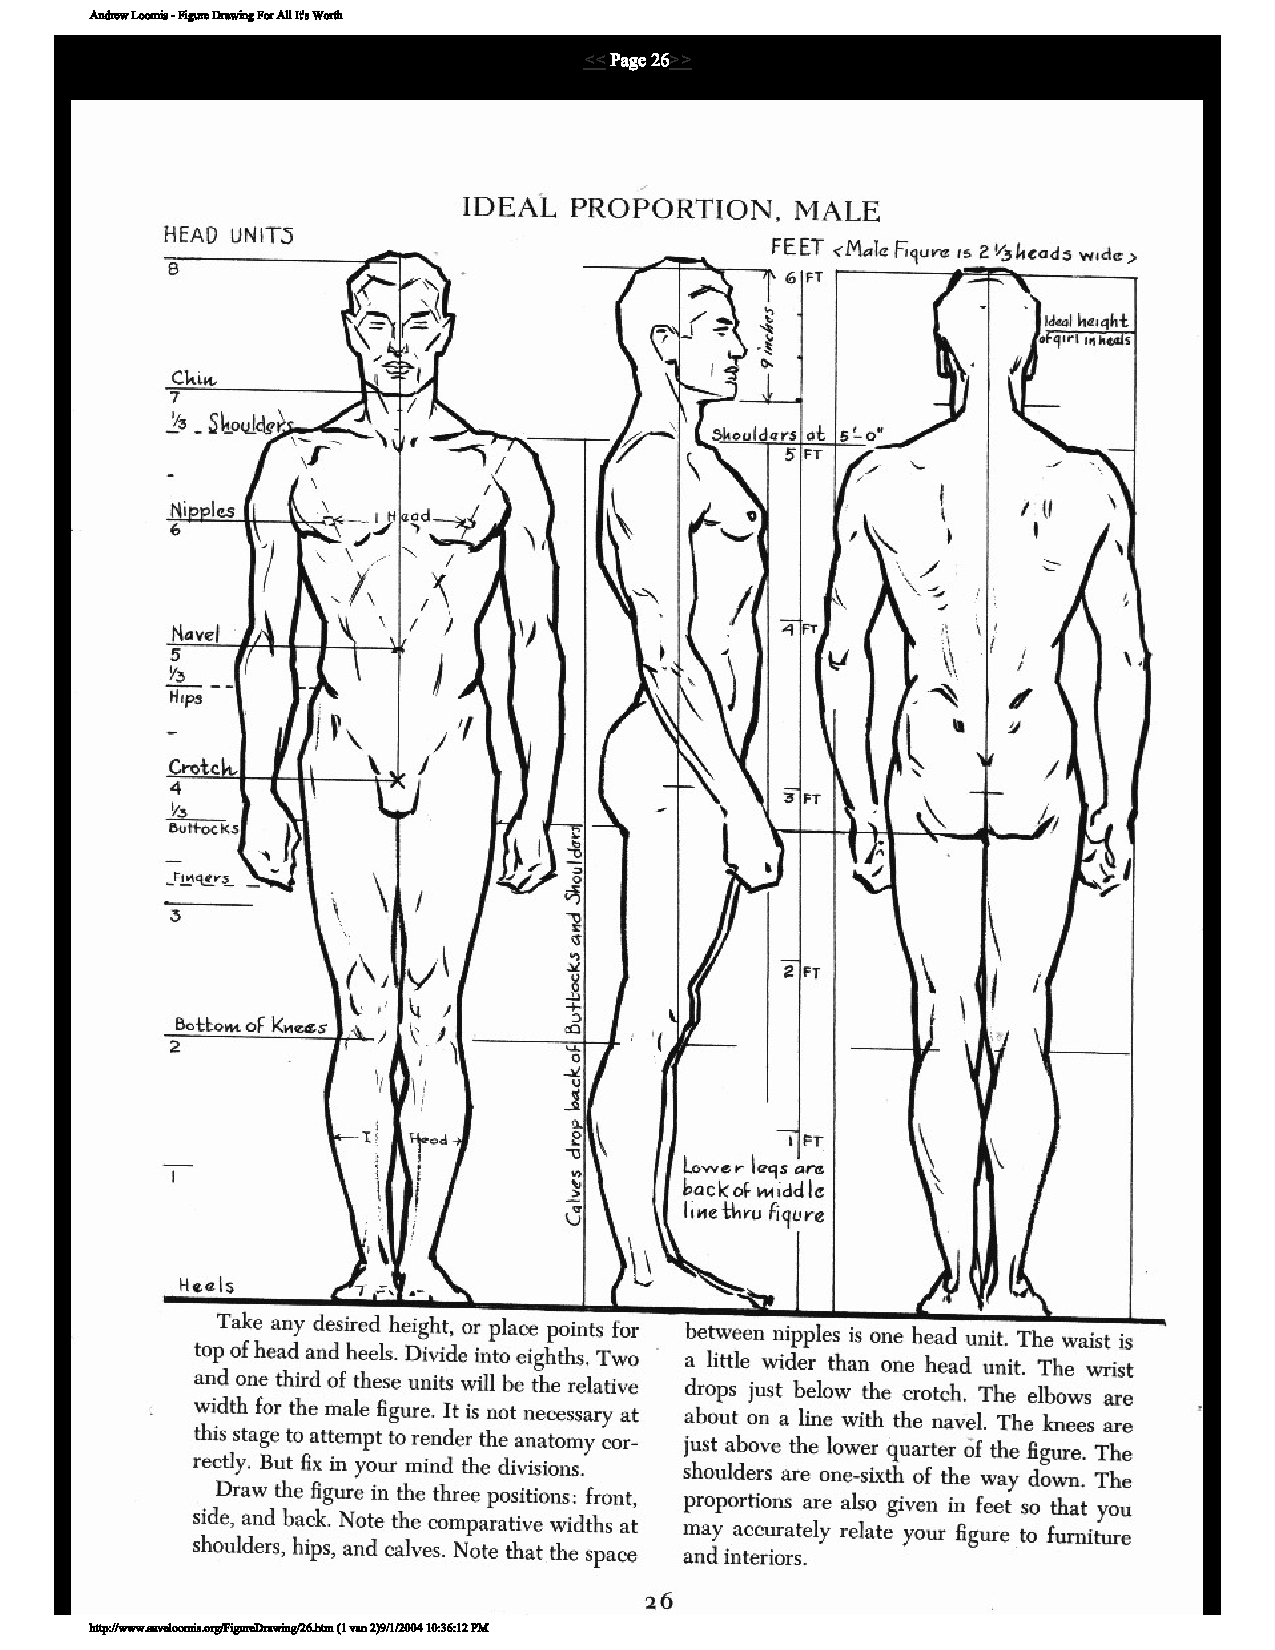
\includegraphics{figures/Loomis1.pdf}
        \caption{ \citet{harris:2000} }
        \label{fig:sub-first}
    \end{subfigure}
    \begin{subfigure}[h]{0.5\textwidth}
    \centering
        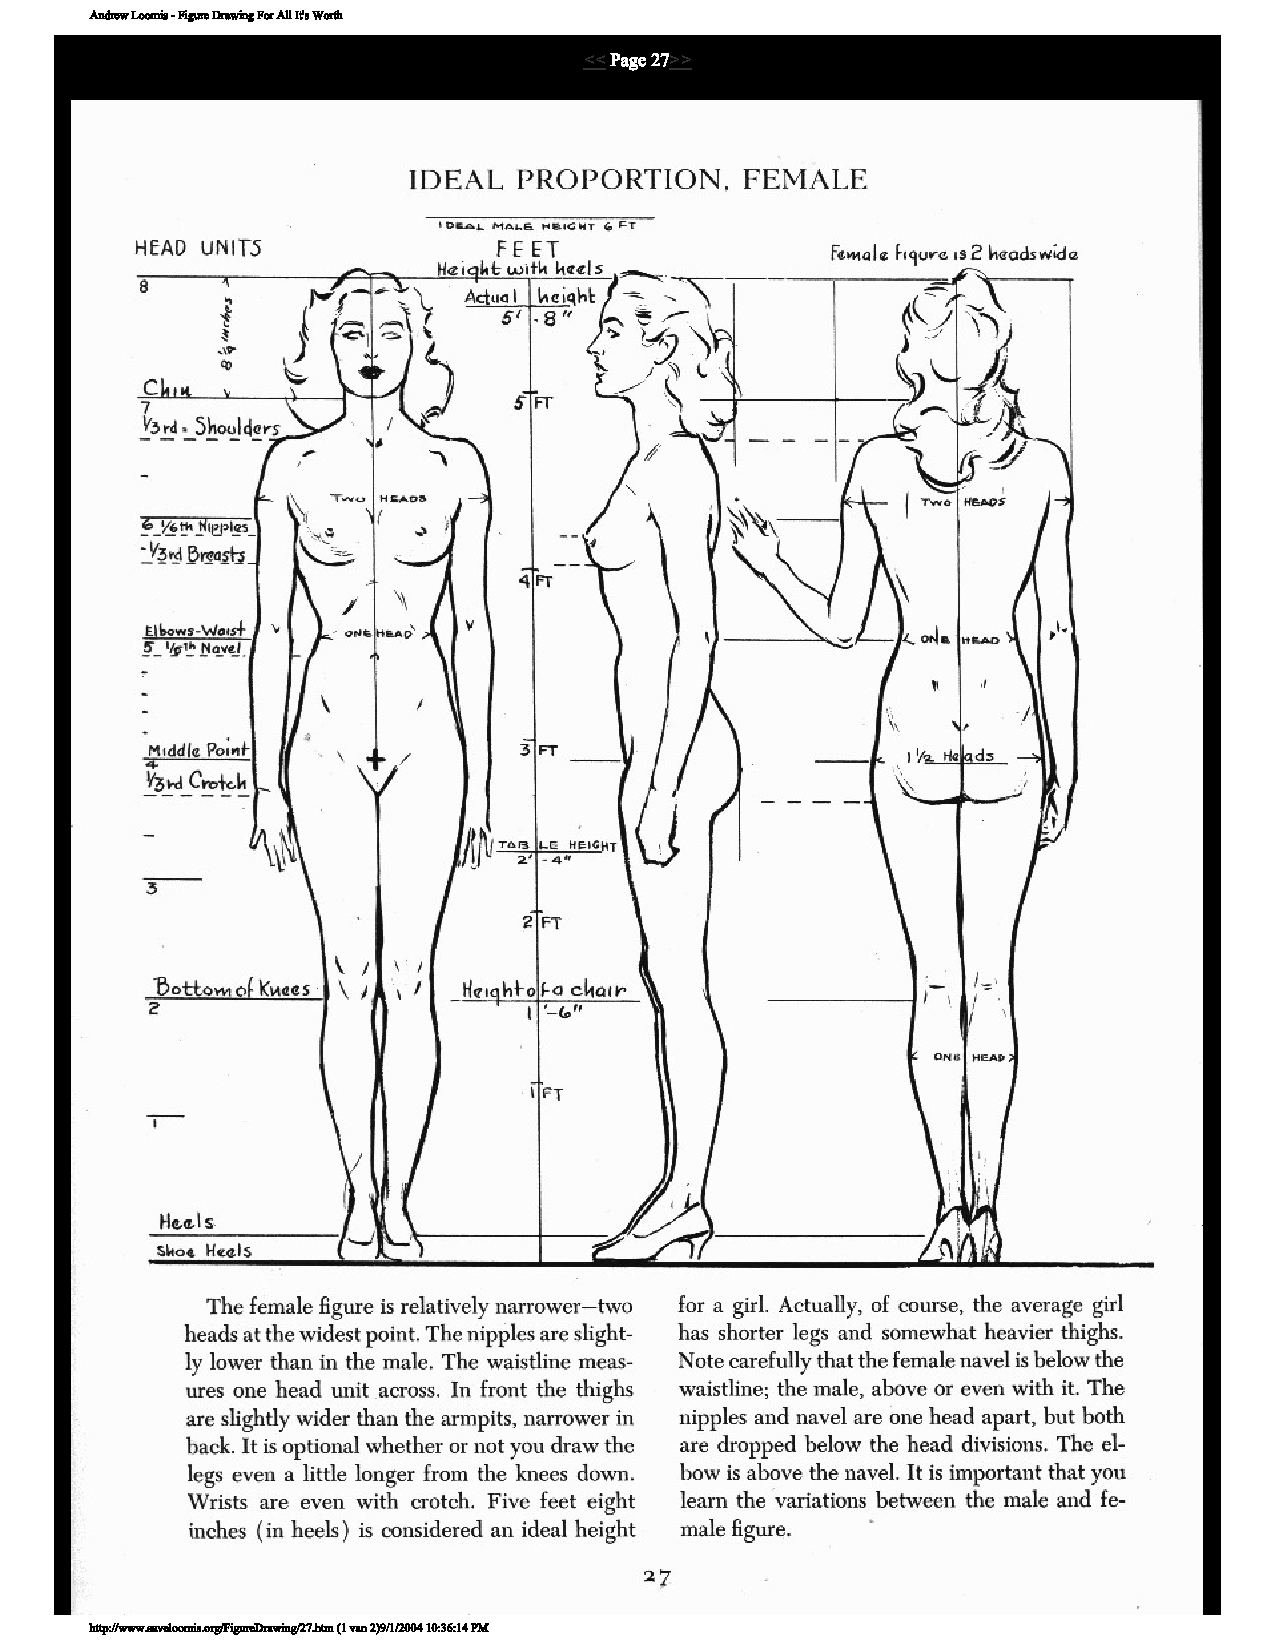
\includegraphics{figures/Loomis2.pdf}
            \caption{\citet{harris:2000}}
        \label{fig:sub-second}
    \end{subfigure}
    \vspace{2.5mm}
    \hrule
    \vspace{2.5mm}
        \caption{ }
        \label{fig:combined}
    \vspace{-2.5mm}
    \hrule
\end{figure}

\section{Primary research question}
\label{sec:rq}

Were the idealized body proportions proposed by Loomis accurate?

\subsection{Secondary question}
\label{sec:rq2}

Do these proportions hold true for both male and female populations?

\subsection{Tertiary question}
\label{sec:rq3}

Are there other proportion ``rules'' that can be inferred from the data?

\section{Data Description}
\label{sec:data}

Data was collected from WSU students as part of a course in Multivariate
Statistics. Each student was responsible for submitting body
measurements and metadata from 10 unique people. Students created a hand
out and requested measurements of different body parts from both the
left and right hand sides, as well as categorical data regarding eye
color, dominant writing hand, ethnicity, and other covariates. The
student data submissions were aggregated and then anonymized and
screened for duplicate or low-integrity entries. The initial dataset of
428 samples was reduced to 251 individuals ranging in age from 1 to 94
years old. Since body proportions change from juveniles through
adulthood, the data set was further constrained to include only adults
18 years of age or older, leaving a pool of 223 individuals. Loomis
maintained that the same ratio applied to both males and females, so
subjects from both genders were considered.

Participants were expected to measure themselves and were asked to rate
the quality their measurements. While both left and right sides body
parts were requested, the difference in recorded length attributable to
asymmetry was considered to be less than the measurement error.
Therefore, the average of both sides was calculated and submitted.

\subsection{Summary of Sample}
\label{sec:data-sample}

Approximately 47\% or respondents were female, 53\% were male, and less
than 1\% identified as non binary. The average age of the study
participants was 37, while the median age was 29. The ethnicity of the
participants surveyed was 73.5\% Caucasian, 17\% Asian, 3.1\% Hispanic,
1.3\% African American, 3.1\% mixed race, and 1.8\% were members of
other races.

\subsection{Summary Statistics of Data}
\label{sec:data-summary}

A Kaiser-Meyer-Olkin (KMO) Test was performed and confirmed the data was
suitable for factor analysis. The data was then scaled and a correlation
table was prepared to for total height and head height (Table 1). A
correlation table showing all the measurements was also prepared and has
been included in the Appendix.

\begin{table}[!htbp]
\footnotesize
\centering
\caption{\textbf{Descriptive Statistics and Correlation Analysis}}
\label{table:correlation}
\begin{tabularx}{1.1\textwidth}{{r@{ \ \ } p{35mm} r@{}lp{1mm} r@{}l p{5mm} r@{}l p{2mm} r@{}l p{2mm} r@{}l p{2mm}   r@{}l  }}
 & \\
\hline
 & \\
\multicolumn{2}{c}{\textbf{ }} & \multicolumn{2}{c}{\textbf{M}} & & \multicolumn{2}{c}{\textbf{SD}} &  & \multicolumn{2}{c}{\textbf{1}} &  & \multicolumn{2}{c}{\textbf{2}} &  & \multicolumn{2}{c}{\textbf{3}} &  & \\ 
 & \\
\hline
 & \\
\textbf{1} & \textbf{Total Height (in)} &  &.0 &  &  1&.00 &  &  1&  &  &  \multicolumn{2}{c}{ \  \  \  \  \ }  &  &  \multicolumn{2}{c}{ \  \  \  \  \ }  &  & \\ 
 & \\
\textbf{2} & \textbf{Head Height (in)} &  &.0 &  &  1&.00 &  &  &.18{$^{**}$}  &  &  1&  &  &  \multicolumn{2}{c}{ \  \  \  \  \ }  &  & \\ 
 & \\
\textbf{3} & \textbf{Total Height (in)} &  &.0 &  &  1&.00 &  &  1&.00{$^{***}$}  &  &  &.18{$^{**}$}  &  &  1&  &  & \\ 
 & \\
\textbf{4} & \textbf{Head Height (in} &  &.0 &  &  1&.00 &  &  &.18{$^{**}$}  &  &  1&.00{$^{***}$}  &  &  &.18{$^{**}$}  &  & \\ 
 & \\
\hline
 & \\
\multicolumn{16}{p{0.99\textwidth}}{  \footnotesize { \begin{hangparas}{0.75in}{1} \textbf{\underline{Notes}:} \ \ Pearson pairwise correlations are reported; \newline a two-side test was performed to report correlation significance.  \end{hangparas} } }  & \\  
\multicolumn{16}{p{0.99\textwidth}}{  {\tiny {$^{\dagger} p < .10$} }  {     } {\tiny        {$^{*} p < .05$} }  {     } {\tiny       {$^{**} p < .01$} }  {     } {\tiny      {$^{***} p < .001$} } {     }     } & \\ 
 & \\
\hline
\end{tabularx}
\end{table}


\section{Key Findings}
\label{sec:findings}

Height was found to have a strong positive correlation with the armpit
to floor measurement (Appendix: Table 1). Head height and overall
height, however, were not shown to have a strong correlation (Table 1).
To further investigate the accuracy of Loomis's ideal body proportions,
each individual survey respondents height was divided by 8, and that
number was compared to the actual head height measurement. The 1/8th
total height approximation for head height was found to have one
standard deviation equal to +/- 10\% for the data for both genders. When
each gender was examined separately, the standard deviation for males
was 10.16092\% and for females was found to be 10.84867\%, showing
females have a slightly wider variation from the mean than males.

\section{Conclusion}
\label{sec:conclusion}

While Loomis's ideal body proportions may form a useful baseline for
drawing the human body, our study showed that the participants in the
sample population did not to conform to the idealized standard. This
finding was shown to hold true regardless of gender, as neither gender
appears to closely conform to the standard proportions proposed by
Loomis. From analysis of the correlation table, other proportional
``rules'' that could be inferred follow intuitive logic. For example,
total height was shown to be strongly correlated with the floor to
armpit measurement. Foot length, floor to knee distance, floor to hip,
and lower arm length showed a moderate positive correlation.

\newpage
\section{APPENDICES}
\label{sec:appendix}

\subsection{Data Provenance}
\label{sec:appendix-data-provenance}

\newpage
\subsubsection{Data Collection Handout}
\label{sec:appendix-data-handout}

\begin{figure}[!ht]
    \hrule
    \caption{ \textbf{Handout Page 1} }
    \begin{center}
        \scalebox{1.00}{    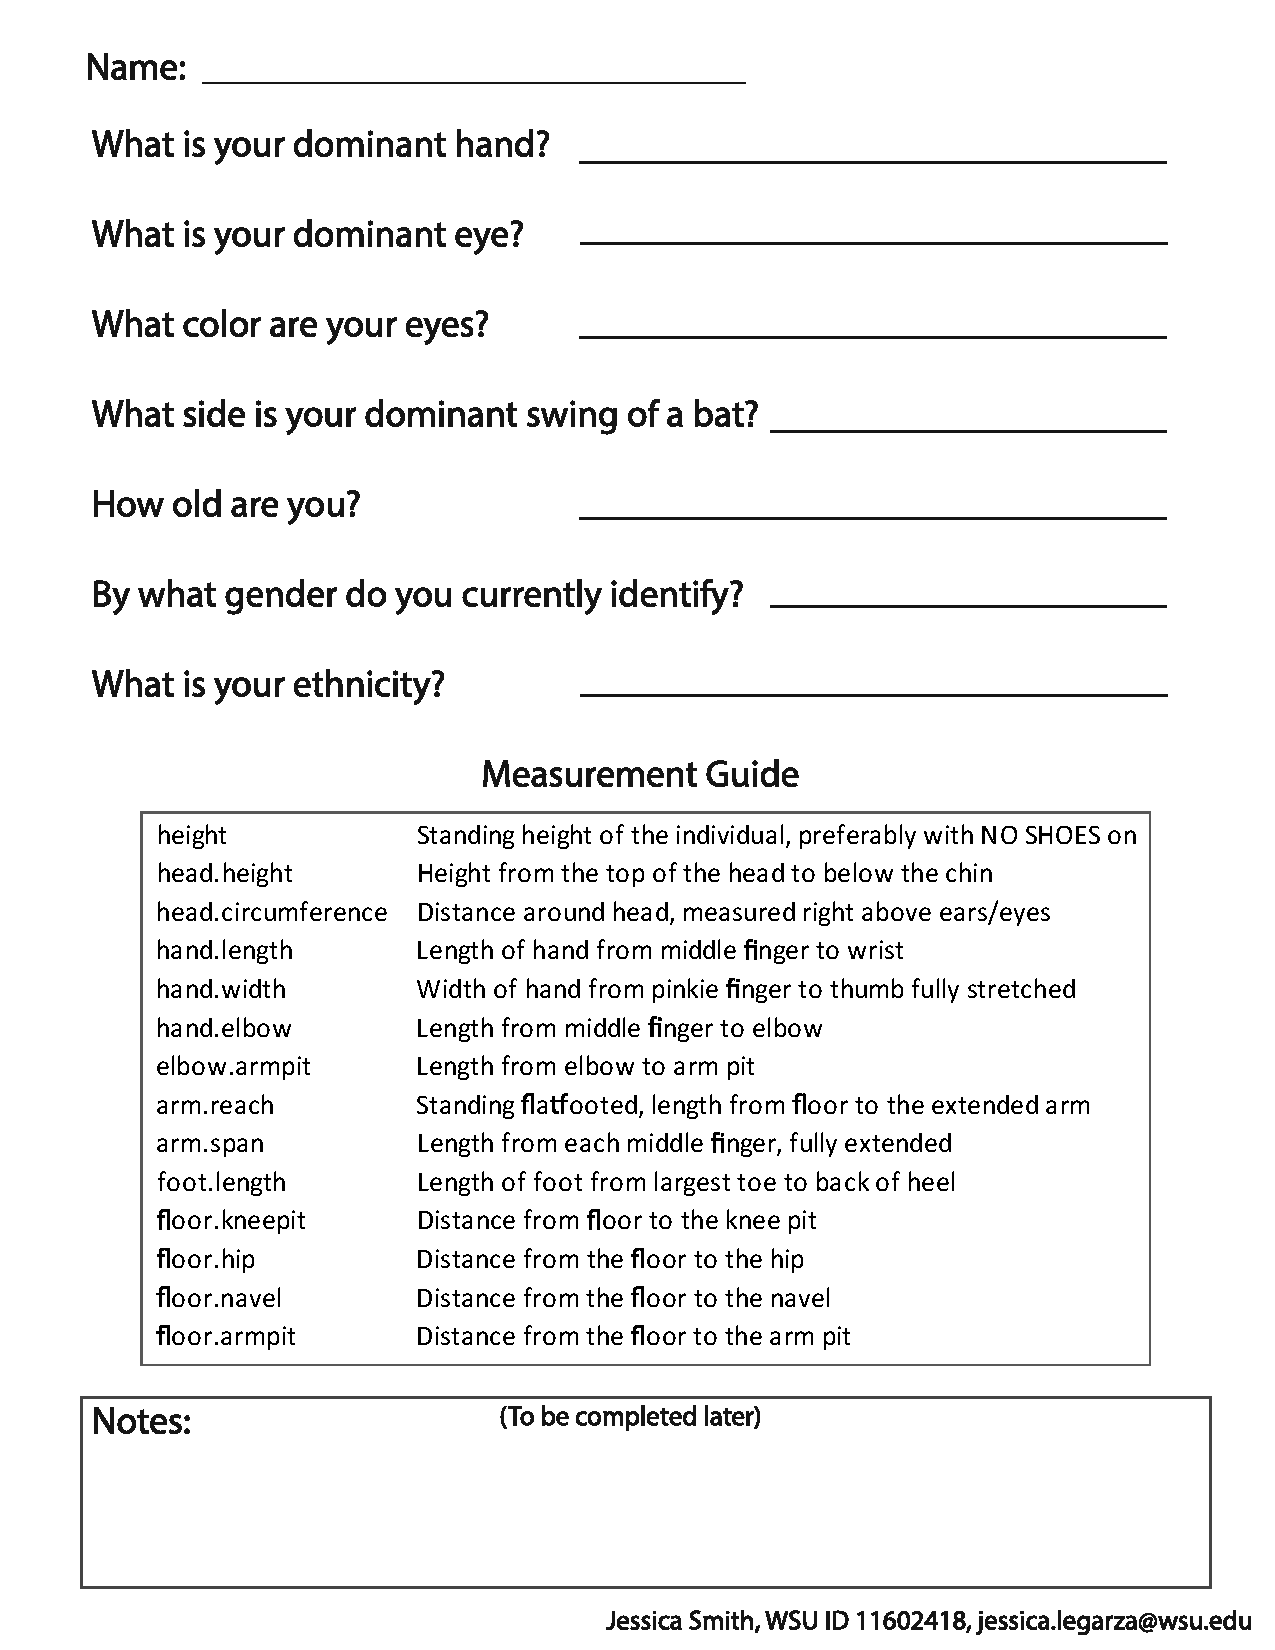
\includegraphics[trim = 0 0 0 0,clip,width=0.85\textwidth]{pdfs/handout1.pdf} }
    \end{center}
    \label{fig:handout-1}
    \hrule
\end{figure}

\newpage

\begin{figure}[!ht]
    \hrule
    \caption{ \textbf{Handout Page 2} }
    \begin{center}
        \scalebox{1.00}{    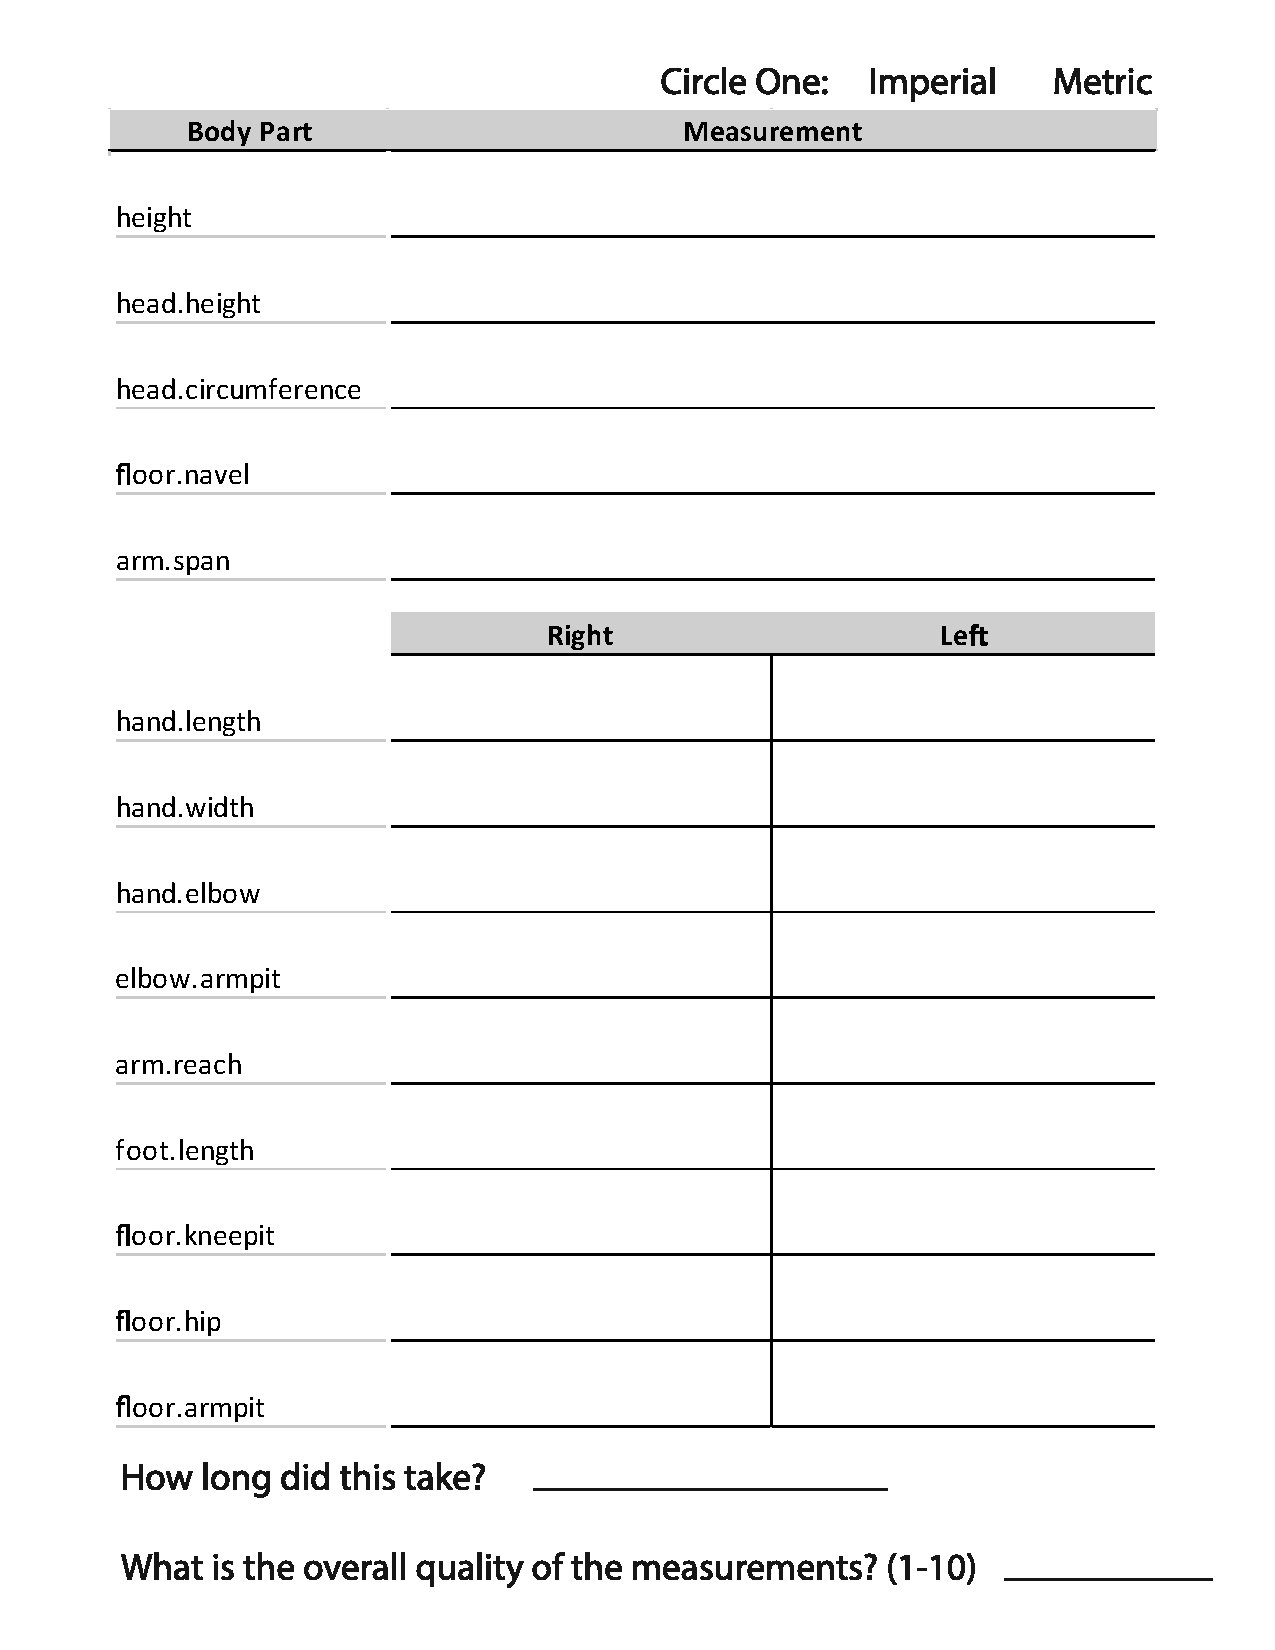
\includegraphics[trim = 0 0 0 0,clip,width=0.85\textwidth]{pdfs/handout2.pdf} }
    \end{center}
    \label{fig:handout-2}
    \hrule
\end{figure}

\newpage

\newpage
\subsubsection{Full Correlation Table}
\label{sec:appendix-corr-table}

\begin{figure}[!ht]
    \hrule
    \caption{ \textbf{Correlation Table} }
    \begin{center}
        \scalebox{1.00}{    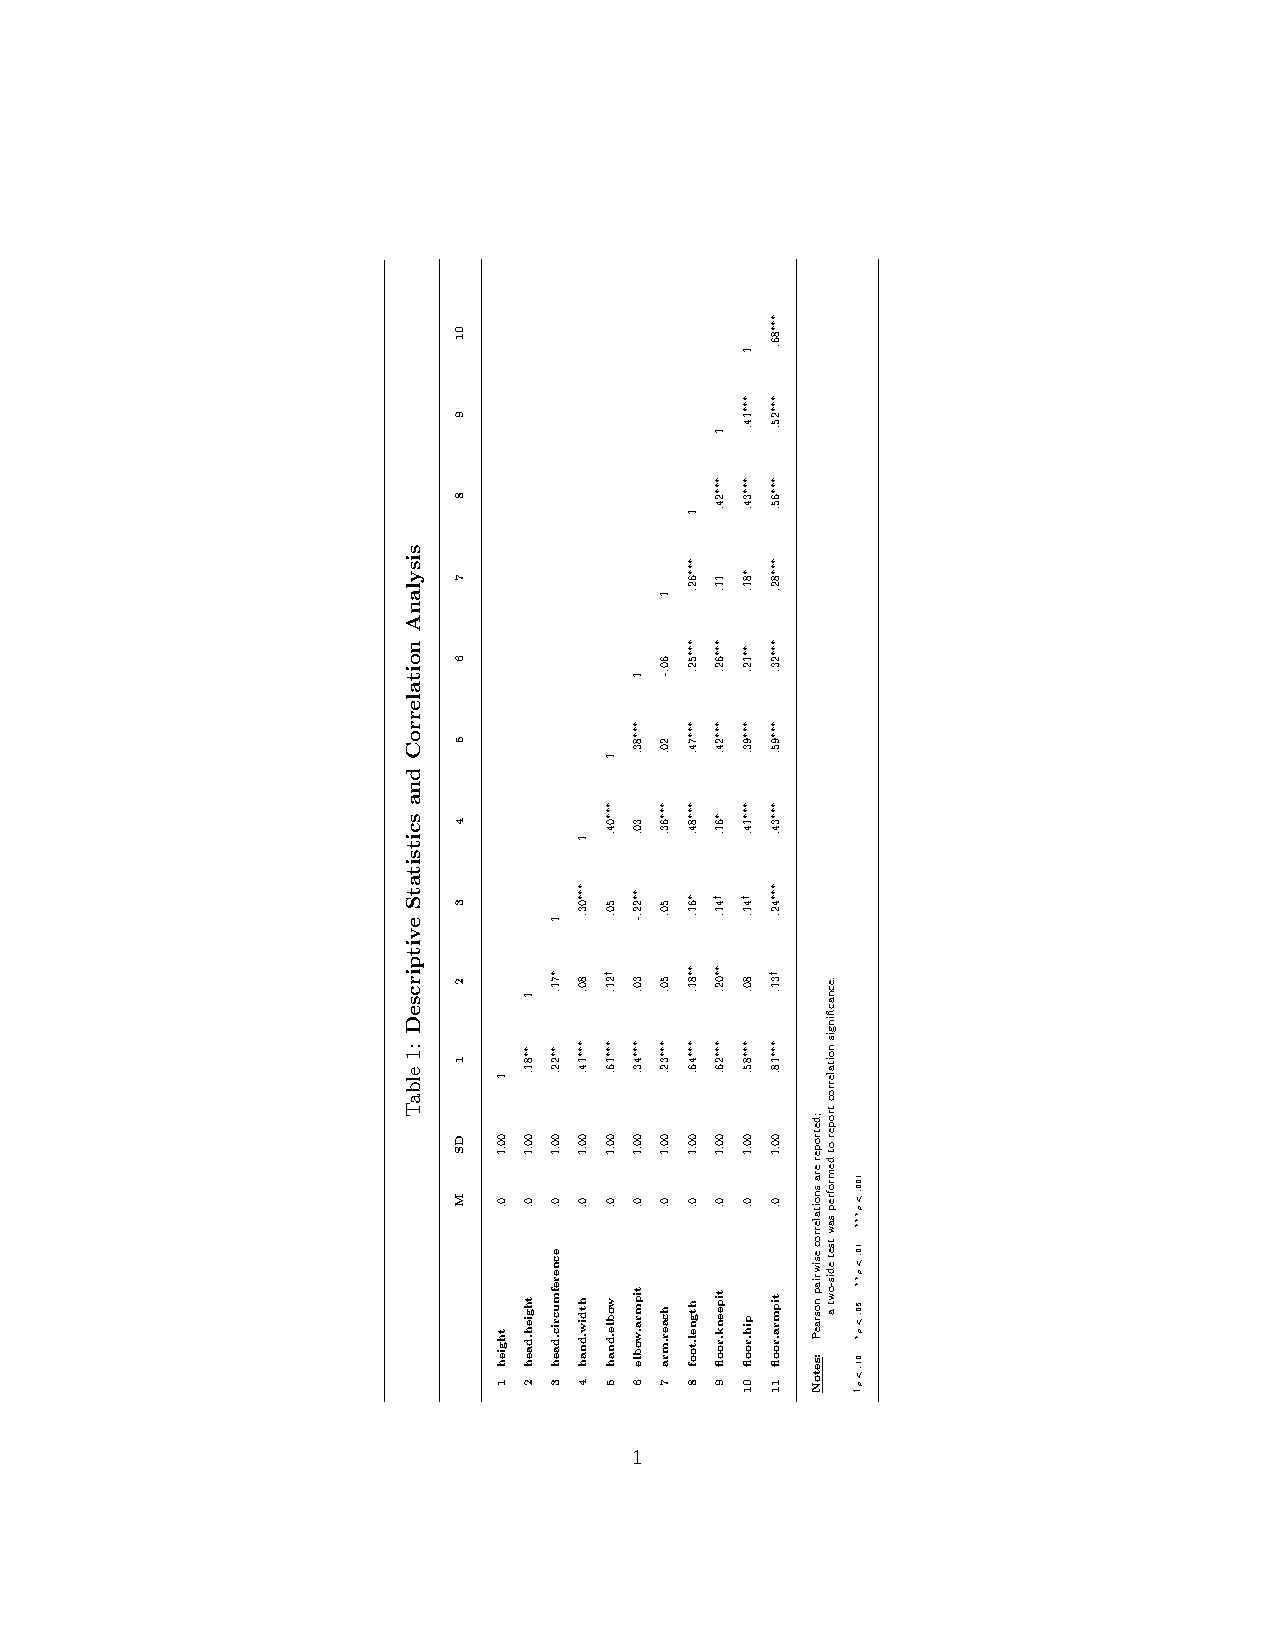
\includegraphics[trim = 0 0 0 0,clip,width=0.85\textwidth]{pdfs/Corr_table_large.pdf} }
    \end{center}
    \label{fig:correlation}
    \hrule
\end{figure}

\newpage

\newpage

\subsection{Preparing the Report Workspace as a subsection}
\label{sec:appendix-setup}

\subsubsection{Preparing the Report Workspace as a subsubsection}
\label{sec:appendix-setup2}

\paragraph{Preparing the Report Workspace as a paragraph}
\label{sec:appendix-setup3}

\subparagraph{Preparing the Report Workspace as a subparagrah}
\label{sec:appendix-setup4}

Below is the necessary functions and libraries required to run the code
referenced in this document.

\begin{Shaded}
\begin{Highlighting}[]
\KeywordTok{library}\NormalTok{(devtools);       }\CommentTok{\# required for source\_url}
\end{Highlighting}
\end{Shaded}

\begin{verbatim}
## Warning: package 'devtools' was built under R version 4.0.3
\end{verbatim}

\begin{Shaded}
\begin{Highlighting}[]
\NormalTok{path.humanVerseWSU =}\StringTok{ "https://raw.githubusercontent.com/MonteShaffer/humanVerseWSU/"}
\KeywordTok{source\_url}\NormalTok{( }\KeywordTok{paste0}\NormalTok{(path.humanVerseWSU,}\StringTok{"master/misc/functions{-}project{-}measure.R"}\NormalTok{) );}
\end{Highlighting}
\end{Shaded}

\begin{verbatim}
## Warning: package 'survival' was built under R version 4.0.3
\end{verbatim}

Below is the code to load the data and prepare it for analysis.

\begin{Shaded}
\begin{Highlighting}[]
\NormalTok{path.project =}\StringTok{ "C:}\CharTok{\textbackslash{}\textbackslash{}}\StringTok{Users}\CharTok{\textbackslash{}\textbackslash{}}\StringTok{jsmit}\CharTok{\textbackslash{}\textbackslash{}}\StringTok{Desktop}\CharTok{\textbackslash{}\textbackslash{}}\StringTok{WSU}\CharTok{\textbackslash{}\textbackslash{}}\StringTok{DataAnalytics}\CharTok{\textbackslash{}\textbackslash{}}\StringTok{STAT419}\CharTok{\textbackslash{}\textbackslash{}}
\StringTok{WSU\_STATS419\_FALL2020}\CharTok{\textbackslash{}\textbackslash{}}\StringTok{project{-}measure}\CharTok{\textbackslash{}\textbackslash{}}\StringTok{"}\NormalTok{;}


\NormalTok{path.to.secret =}\StringTok{ "C:}\CharTok{\textbackslash{}\textbackslash{}}\StringTok{Users}\CharTok{\textbackslash{}\textbackslash{}}\StringTok{jsmit}\CharTok{\textbackslash{}\textbackslash{}}\StringTok{Desktop}\CharTok{\textbackslash{}\textbackslash{}}\StringTok{WSU}\CharTok{\textbackslash{}\textbackslash{}}\StringTok{DataAnalytics}\CharTok{\textbackslash{}\textbackslash{}}\StringTok{STAT419}\CharTok{\textbackslash{}\textbackslash{}}\StringTok{\_SECRET\_}\CharTok{\textbackslash{}\textbackslash{}}\StringTok{"}\NormalTok{;}

\NormalTok{measure =}\StringTok{ }\NormalTok{utils}\OperatorTok{::}\KeywordTok{read.csv}\NormalTok{( }\KeywordTok{paste0}\NormalTok{(path.to.secret, }\StringTok{"measure{-}students.txt"}\NormalTok{), }
                           \DataTypeTok{header=}\OtherTok{TRUE}\NormalTok{, }\DataTypeTok{quote=}\StringTok{""}\NormalTok{, }\DataTypeTok{sep=}\StringTok{"|"}\NormalTok{);}

\NormalTok{path.github =}\StringTok{ "https://raw.githubusercontent.com/jsmith0434/WSU\_STATS419\_FALL2020"}\NormalTok{;}
\KeywordTok{source\_url}\NormalTok{( }\KeywordTok{paste0}\NormalTok{(path.github,}\StringTok{"/master/functions/functions{-}project.R"}\NormalTok{) );}

\NormalTok{measure\_data =}\StringTok{ }\NormalTok{utils}\OperatorTok{::}\KeywordTok{read.csv}\NormalTok{( }\KeywordTok{paste0}\NormalTok{(path.to.secret, }\StringTok{"final.measure.txt"}\NormalTok{), }
                                \DataTypeTok{header=}\OtherTok{TRUE}\NormalTok{, }\DataTypeTok{quote=}\StringTok{""}\NormalTok{, }\DataTypeTok{sep=}\StringTok{"|"}\NormalTok{);}
\NormalTok{measure\_cleaned =}\StringTok{ }\KeywordTok{cleanUpData}\NormalTok{(measure\_data)}

\NormalTok{adults =}\StringTok{ }\NormalTok{measure\_cleaned[measure\_cleaned}\OperatorTok{$}\NormalTok{age }\OperatorTok{\textgreater{}=}\StringTok{ }\DecValTok{18}\NormalTok{, ]}
\end{Highlighting}
\end{Shaded}

Below is the code to generate the summary statistics and save them as
the table that you see in Section \ref{}.

\begin{Shaded}
\begin{Highlighting}[]
\NormalTok{path.humanVerseWSU =}\StringTok{ "https://raw.githubusercontent.com/MonteShaffer/humanVerseWSU/"}
\KeywordTok{source\_url}\NormalTok{( }\KeywordTok{paste0}\NormalTok{(path.humanVerseWSU,}\StringTok{"master/misc/functions{-}project{-}measure.R"}\NormalTok{) );}

\NormalTok{path.project =}\StringTok{ "C:}\CharTok{\textbackslash{}\textbackslash{}}\StringTok{Users}\CharTok{\textbackslash{}\textbackslash{}}\StringTok{jsmit}\CharTok{\textbackslash{}\textbackslash{}}\StringTok{Desktop}\CharTok{\textbackslash{}\textbackslash{}}\StringTok{WSU}\CharTok{\textbackslash{}\textbackslash{}}\StringTok{DataAnalytics}\CharTok{\textbackslash{}\textbackslash{}}\StringTok{STAT419}\CharTok{\textbackslash{}\textbackslash{}}
\StringTok{WSU\_STATS419\_FALL2020}\CharTok{\textbackslash{}\textbackslash{}}\StringTok{project{-}measure}\CharTok{\textbackslash{}\textbackslash{}}\StringTok{"}\NormalTok{;}
\NormalTok{path.tables =}\StringTok{ }\KeywordTok{paste0}\NormalTok{(path.project,}\StringTok{"tables}\CharTok{\textbackslash{}\textbackslash{}}\StringTok{"}\NormalTok{);}

\NormalTok{file.correlation =}\StringTok{ }\KeywordTok{paste0}\NormalTok{(path.tables,}\StringTok{"height{-}head{-}correlation{-}table.tex"}\NormalTok{);}

\NormalTok{myData =}\StringTok{ }\KeywordTok{as.matrix}\NormalTok{(adults[, }\DecValTok{3}\OperatorTok{:}\DecValTok{4}\NormalTok{]);  }\CommentTok{\# numeric values only, only what will appear in table}
\NormalTok{myData =}\StringTok{ }\KeywordTok{scale}\NormalTok{(myData)}
\NormalTok{myData =}\StringTok{ }\KeywordTok{cbind}\NormalTok{(myData,myData);}

\KeywordTok{buildLatexCorrelationTable}\NormalTok{(myData, }
  \DataTypeTok{rotateTable =} \OtherTok{FALSE}\NormalTok{,}
  \DataTypeTok{width.table =} \FloatTok{01.1}\NormalTok{,}
  \DataTypeTok{myFile =}\NormalTok{ file.correlation,}
  \DataTypeTok{myNames =} \KeywordTok{c}\NormalTok{(}\StringTok{"Total Height (in)"}\NormalTok{, }\StringTok{"Head Height (in)"}\NormalTok{, }\StringTok{"Total Height (in)"}\NormalTok{, }\StringTok{"Head Height (in"}\NormalTok{) );}

\KeywordTok{Sys.sleep}\NormalTok{(}\DecValTok{2}\NormalTok{); }\CommentTok{\# in case Knit{-}PDF doesn\textquotesingle{}t like that I just created the file...}
\end{Highlighting}
\end{Shaded}

A pie chart showing the breakdown of participants by gender.

\begin{Shaded}
\begin{Highlighting}[]
\NormalTok{mytable2 \textless{}{-}}\StringTok{ }\KeywordTok{table}\NormalTok{(adults}\OperatorTok{$}\NormalTok{gender)}
\NormalTok{lbls \textless{}{-}}\StringTok{ }\KeywordTok{paste}\NormalTok{(}\KeywordTok{names}\NormalTok{(mytable2), }\StringTok{": "}\NormalTok{, mytable2, }\DataTypeTok{sep=}\StringTok{""}\NormalTok{)}
\KeywordTok{pie}\NormalTok{(mytable2, }\DataTypeTok{labels =}\NormalTok{ lbls,  }\DataTypeTok{main=}\StringTok{"Respondent Gender"}\NormalTok{)}
\end{Highlighting}
\end{Shaded}

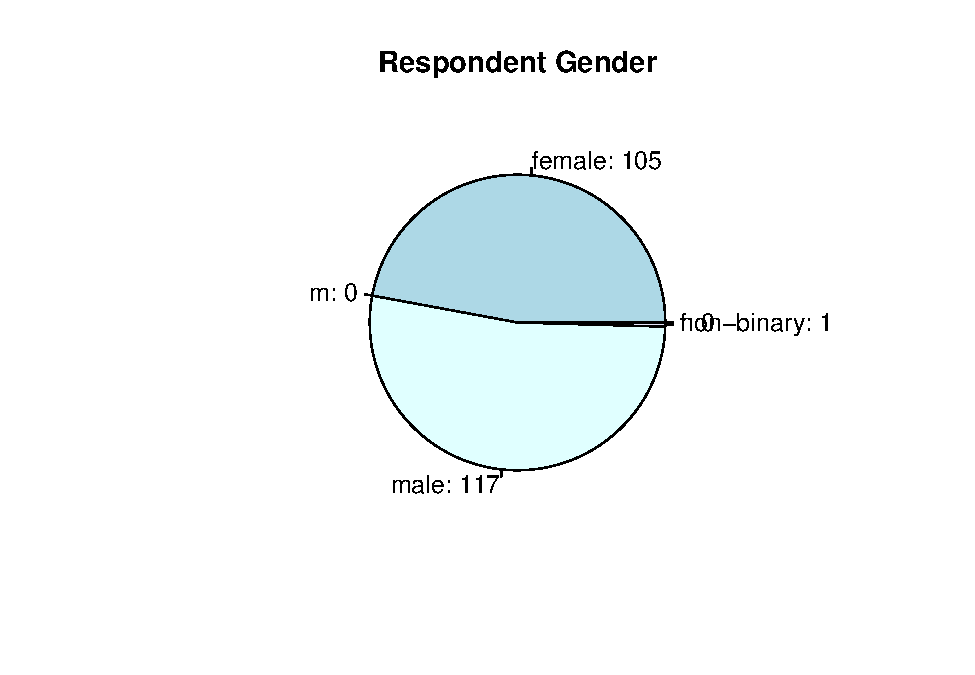
\includegraphics{project-measure-writeup-student_files/figure-latex/unnamed-chunk-1-1.pdf}

A pie chart showing ethnicity.

\begin{Shaded}
\begin{Highlighting}[]
\NormalTok{mytable \textless{}{-}}\StringTok{ }\KeywordTok{round}\NormalTok{(}\KeywordTok{prop.table}\NormalTok{(}\KeywordTok{table}\NormalTok{(adults}\OperatorTok{$}\NormalTok{ethnicity))}\OperatorTok{*}\DecValTok{100}\NormalTok{,}\DecValTok{1}\NormalTok{)}
\NormalTok{lbls \textless{}{-}}\StringTok{ }\KeywordTok{paste}\NormalTok{(}\KeywordTok{names}\NormalTok{(mytable), }\StringTok{": "}\NormalTok{, mytable, }\DataTypeTok{sep=}\StringTok{""}\NormalTok{)}
\KeywordTok{pie}\NormalTok{(mytable, }\DataTypeTok{labels =}\NormalTok{ lbls,   }\DataTypeTok{main=}\StringTok{"Respondent Ethicity"}\NormalTok{)}
\end{Highlighting}
\end{Shaded}

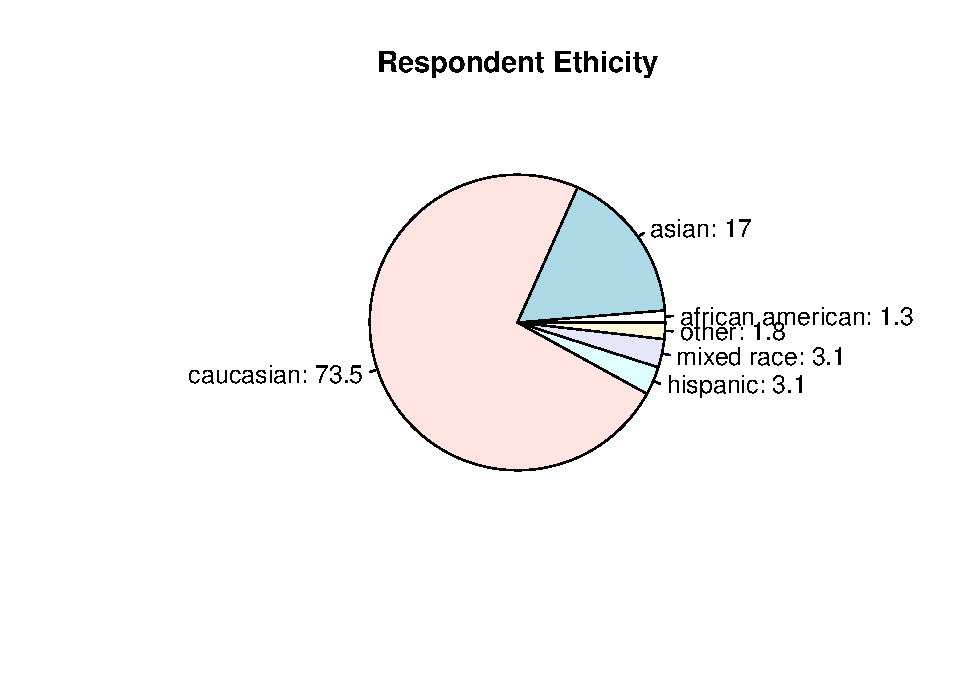
\includegraphics{project-measure-writeup-student_files/figure-latex/unnamed-chunk-2-1.pdf}

Histograms that show the distribution of the percent deviation from the
ideal standard head height to body height ratio proposed by Loomis.

\begin{Shaded}
\begin{Highlighting}[]
\NormalTok{sub =}\StringTok{ }\NormalTok{adults[, }\KeywordTok{c}\NormalTok{(}\StringTok{"height"}\NormalTok{, }\StringTok{"head.height"}\NormalTok{, }\StringTok{"gender"}\NormalTok{)]}
\NormalTok{sub}\OperatorTok{$}\NormalTok{eighth =}\StringTok{ }\NormalTok{sub}\OperatorTok{$}\NormalTok{height}\OperatorTok{/}\DecValTok{8} 
\NormalTok{sub}\OperatorTok{$}\NormalTok{percent\_diff =}\StringTok{ }\NormalTok{((sub}\OperatorTok{$}\NormalTok{head.height }\OperatorTok{{-}}\StringTok{ }\NormalTok{sub}\OperatorTok{$}\NormalTok{eighth)}\OperatorTok{/}\NormalTok{sub}\OperatorTok{$}\NormalTok{head.height) }\OperatorTok{*}\StringTok{ }\DecValTok{100}

\KeywordTok{hist}\NormalTok{(sub}\OperatorTok{$}\NormalTok{percent\_diff[sub}\OperatorTok{$}\NormalTok{gender}\OperatorTok{==}\StringTok{"female"}\NormalTok{])}
\end{Highlighting}
\end{Shaded}

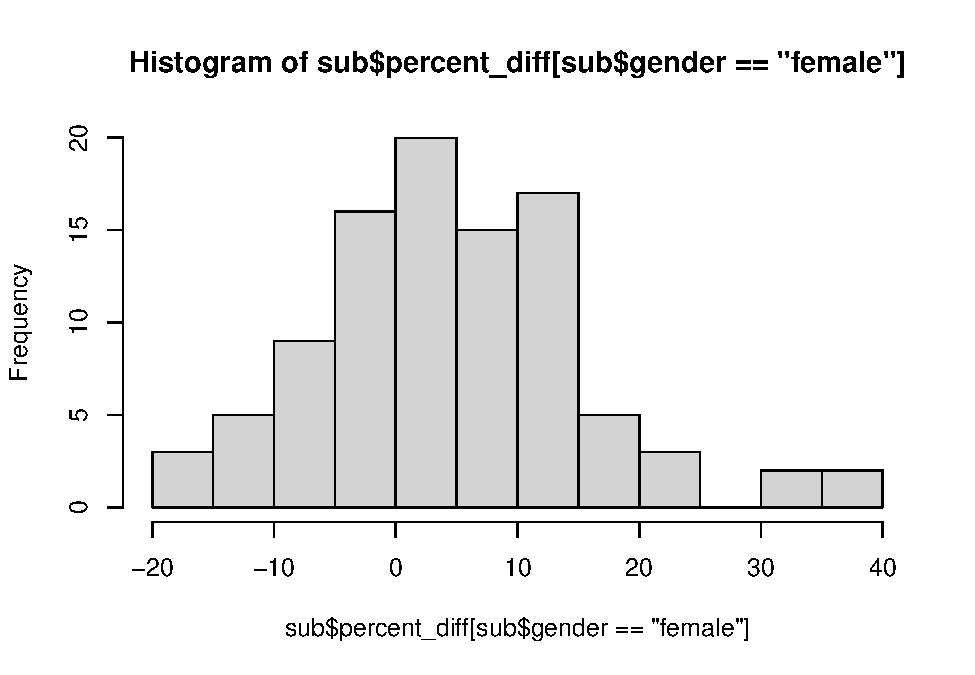
\includegraphics{project-measure-writeup-student_files/figure-latex/unnamed-chunk-3-1.pdf}

\begin{Shaded}
\begin{Highlighting}[]
\KeywordTok{hist}\NormalTok{(sub}\OperatorTok{$}\NormalTok{percent\_diff[sub}\OperatorTok{$}\NormalTok{gender}\OperatorTok{==}\StringTok{"male"}\NormalTok{])}
\end{Highlighting}
\end{Shaded}

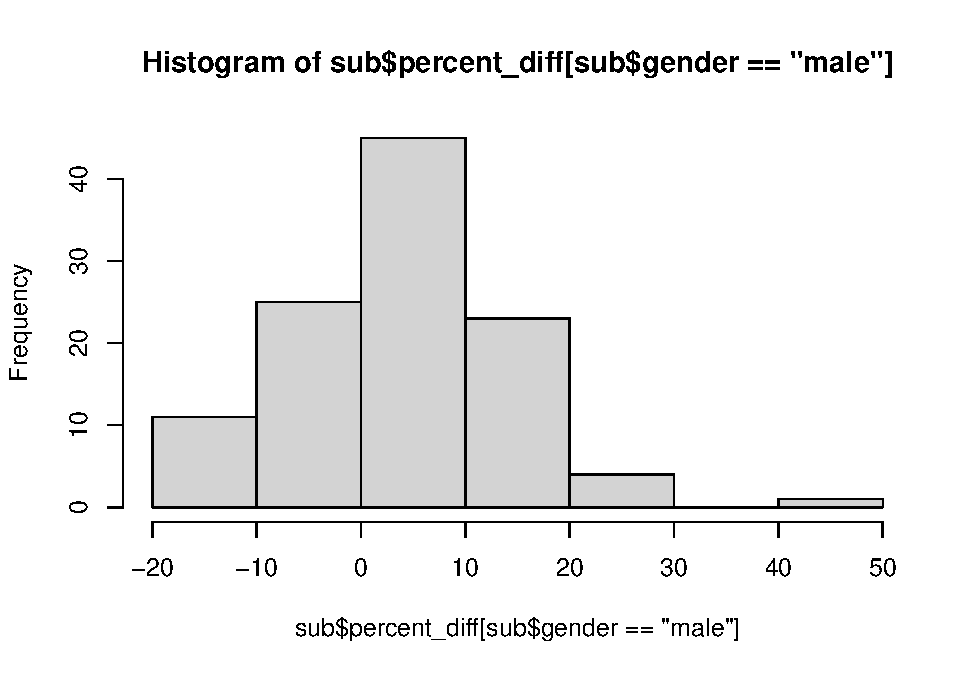
\includegraphics{project-measure-writeup-student_files/figure-latex/unnamed-chunk-3-2.pdf}

\begin{Shaded}
\begin{Highlighting}[]
\KeywordTok{hist}\NormalTok{(sub}\OperatorTok{$}\NormalTok{percent\_diff)}
\end{Highlighting}
\end{Shaded}

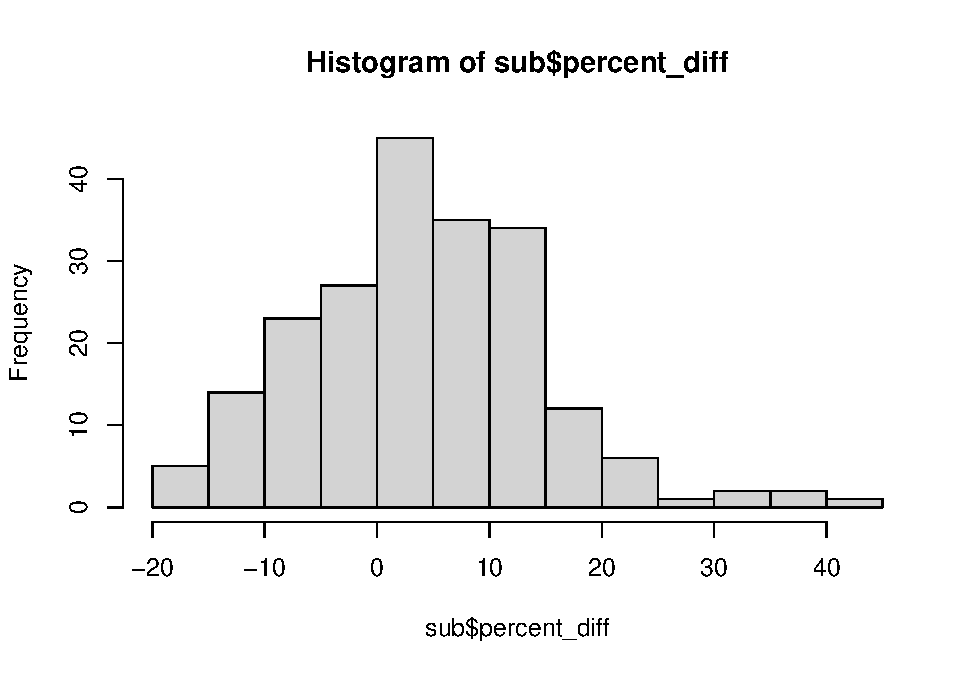
\includegraphics{project-measure-writeup-student_files/figure-latex/unnamed-chunk-3-3.pdf}

The code used to generate the KMO score.

\begin{Shaded}
\begin{Highlighting}[]
\NormalTok{sub2 =}\StringTok{ }\NormalTok{adults[ ,}\KeywordTok{c}\NormalTok{(}\DecValTok{3}\NormalTok{,}\DecValTok{4}\NormalTok{,}\DecValTok{5}\NormalTok{,}\DecValTok{20}\OperatorTok{:}\DecValTok{27}\NormalTok{)]}
\NormalTok{sub2 =}\StringTok{ }\KeywordTok{scale}\NormalTok{(sub2)}
\NormalTok{sub2 =}\StringTok{ }\KeywordTok{as.data.frame}\NormalTok{(sub2)}

\CommentTok{\# this is the standard correlation matrix}
\NormalTok{sub2.corr =}\StringTok{ }\KeywordTok{cor}\NormalTok{(sub2, }\DataTypeTok{use =} \StringTok{"complete.obs"}\NormalTok{);}

\KeywordTok{library}\NormalTok{(REdaS); }\CommentTok{\# install.packages("REdaS", dependencies=TRUE);}
\NormalTok{sub2.KMO =}\StringTok{ }\KeywordTok{KMOS}\NormalTok{(sub2, }\DataTypeTok{use =} \StringTok{"complete.obs"}\NormalTok{);}

\NormalTok{my.kmo =}\StringTok{ }\NormalTok{sub2.KMO}\OperatorTok{$}\NormalTok{KMO;}
\NormalTok{my.kmo}
\end{Highlighting}
\end{Shaded}

The code used to generate the large correlation table included in the
appendix.

\begin{Shaded}
\begin{Highlighting}[]
\NormalTok{myData2 =}\StringTok{ }\KeywordTok{as.matrix}\NormalTok{(sub2)}

\NormalTok{file.correlation =}\StringTok{ }\KeywordTok{paste0}\NormalTok{(path.tables,}\StringTok{"scaled{-}correlation{-}table.tex"}\NormalTok{);}

\KeywordTok{buildLatexCorrelationTable}\NormalTok{(myData2, }
  \DataTypeTok{rotateTable =} \OtherTok{TRUE}\NormalTok{,}
  \DataTypeTok{width.table =} \FloatTok{1.6}\NormalTok{,}
  \DataTypeTok{myFile =}\NormalTok{ file.correlation,}
  \DataTypeTok{myNames =} \KeywordTok{c}\NormalTok{(}\KeywordTok{colnames}\NormalTok{(sub2), }\KeywordTok{colnames}\NormalTok{(sub2))}
\NormalTok{)}
\end{Highlighting}
\end{Shaded}





%% appendices go here!


\newpage
\theendnotes

%%%%%%%%%%%%%%%%%%%%%%%%%%%%%%%%%%%  biblio %%%%%%%%
\newpage
\begin{auxmulticols}{1}
\singlespacing 
\bibliography{./biblio/master.bib}

%%%%%%%%%%%%%%%%%%%%%%%%%%%%%%%%%%%  biblio %%%%%%%%
\end{auxmulticols}

\newpage
{
\hypersetup{linkcolor=black}
\setcounter{tocdepth}{3}
\tableofcontents
}



\end{document}